\documentclass[runningheads]{llncs}

\usepackage[T1]{fontenc}        
\usepackage[utf8]{inputenc}     
\usepackage[romanian]{babel}
\usepackage{tcolorbox}          
\tcbuselibrary{skins,breakable}
\usepackage{amsmath}
\usepackage{amsfonts}
\usepackage{amssymb}
\usepackage{hyperref}
\usepackage{listings}
\usepackage{booktabs}
\usepackage{xcolor}
\usepackage{enumitem}
\usepackage{fontawesome5} 
\usepackage{graphicx}
\usepackage{multirow}
\usepackage{array}
\usepackage{float}
\usepackage[
    margin=1.1in
]{geometry}

\definecolor{purple}{HTML}{800080}
\definecolor{red}{HTML}{D00000}
\definecolor{darkblue}{HTML}{000080}
\definecolor{darkgreen}{HTML}{008000}
\definecolor{yellow}{HTML}{FFCC00}
\definecolor{orange}{HTML}{FFA500}
\definecolor{pink}{HTML}{D00080}
\definecolor{teal}{HTML}{008080}
\definecolor{blue}{HTML}{0080D0}
\definecolor{green}{HTML}{00B000}

\tcbset{
    NoteBox/.style={
        breakable,
        arc=3mm,
        boxrule=0.8pt,
        left skip=0pt, right skip=0pt,
        boxsep=2mm, top=2mm, bottom=2mm,
        enhanced, 
    },
    BoxRed/.style={NoteBox, colback=red!10, colframe=red, fonttitle=\bfseries\color{white}},
    BoxDarkBlue/.style={NoteBox, colback=darkblue!10, colframe=darkblue, fonttitle=\bfseries\color{white}},
    BoxDarkGreen/.style={NoteBox, colback=darkgreen!10, colframe=darkgreen, fonttitle=\bfseries\color{white}},
    BoxYellow/.style={NoteBox, colback=yellow!10, colframe=yellow, fonttitle=\bfseries\color{black}},
    BoxOrange/.style={NoteBox, colback=orange!10, colframe=orange, fonttitle=\bfseries\color{black}},
    BoxPink/.style={NoteBox, colback=pink!10, colframe=pink, fonttitle=\bfseries\color{white}},
    BoxTeal/.style={NoteBox, colback=teal!10, colframe=teal, fonttitle=\bfseries\color{white}},
    BoxBlue/.style={NoteBox, colback=blue!10, colframe=blue, fonttitle=\bfseries\color{white}},
    BoxGreen/.style={NoteBox, colback=green!10, colframe=green, fonttitle=\bfseries\color{white}},
    BoxPurple/.style={NoteBox, colback=purple!10, colframe=purple, fonttitle=\bfseries\color{white}}
}

\lstset{
    language=Python,
    basicstyle=\ttfamily\small,
    keywordstyle=\color{purple}\bfseries,
    stringstyle=\color{red},
    commentstyle=\color{darkgreen},
    showstringspaces=false,
    breaklines=true,
    frame=none,
    backgroundcolor=\color{gray!5},  
}

\hypersetup{
    colorlinks=true,
    linkcolor=red,
    urlcolor=blue,
}

\begin{document}

\title{Studiu Comparativ: Problema Bin Packing\\
\large Minimizarea numărului de containere utilizate}
\author{Băran Denis-Constantin\\ Micu Maria-Teodora\\ Epure Roberto-Constantin}
\institute{
Universitatea Națională de Știință și Tehnologie POLITEHNICA București
Analiza Algoritmilor - 2025-2026}
\maketitle

\begin{abstract}
Prezentul raport realizează un studiu comparativ al principalilor algoritmi pentru rezolvarea problemei Bin Packing, o problemă clasică de optimizare combinatorică demonstrat a fi NP-Hard. Am implementat și evaluat șase algoritmi: Next Fit (NF), First Fit (FF), Best Fit (BF), Worst Fit (WF), First Fit Decreasing (FFD) și o soluție optimă bazată pe backtracking cu paralelizare. Experimentele au fost realizate pe 40 de seturi de date cu dimensiuni între 10 și 475 elemente, folosind trei distribuții diferite ale greutăților. Rezultatele demonstrează că FFD oferă cel mai bun compromis între calitatea soluției și timpul de execuție, obținând rezultate foarte apropiate de optim cu complexitate $O(n \log n)$.
\end{abstract}

%==============================================================================
\section{Introducere}
%==============================================================================

Problema Bin Packing reprezintă una dintre cele mai studiate probleme de optimizare combinatorică din informatică. Aceasta apare frecvent în contexte practice precum logistică, alocare de resurse și managementul memoriei.

Formal, problema se enunță astfel: dată fiind o mulțime de $n$ obiecte cu greutăți $w_1, w_2, \ldots, w_n$ și o capacitate maximă $C$ a containerelor (bins), se cere găsirea numărului minim de containere necesare pentru a împacheta toate obiectele, astfel încât suma greutăților din fiecare container să nu depășească $C$.

\subsection{Descrierea Problemei}

Fie o mulțime de $n$ valori și o capacitate maximă reprezentată de numărul natural $C$. Problema constă în partiționarea colecției inițiale într-un număr minim de submulțimi (bins) astfel încât suma valorilor din fiecare submulțime să fie mai mică sau egală cu $C$.

\begin{tcolorbox}[BoxDarkBlue, title=\faIcon{list} Exemplu, fonttitle=\bfseries]
\textbf{Input:} weight[] = [4, 8, 1, 4, 2, 1], C = 10 \\
\textbf{Output:} 2 \\
\textbf{Explicație:} Avem nevoie de minimum 2 containere. Primul container conține [4, 4, 2] (suma = 10), iar al doilea [8, 1, 1] (suma = 10).
\end{tcolorbox}

\subsection{Aplicații Practice}

Problema Bin Packing are numeroase aplicații practice în diverse domenii:

\begin{itemize}
    \item \textbf{Logistică și transport:} Încărcarea mărfurilor în camioane, containere maritime sau avioane, minimizând numărul de vehicule necesare.
    \item \textbf{Industria manufacturieră:} Tăierea materialelor (sticlă, metal, textile) pentru minimizarea deșeurilor.
    \item \textbf{Cloud computing:} Alocarea mașinilor virtuale pe servere fizice pentru maximizarea utilizării resurselor.
    \item \textbf{Managementul memoriei:} Alocarea blocurilor de memorie în sisteme de operare.
    \item \textbf{Planificarea discurilor:} Stocarea fișierelor pe medii de stocare cu capacitate fixă (CD, DVD, hard disk-uri).
    \item \textbf{Programarea sarcinilor:} Distribuirea task-urilor pe procesoare cu constrângeri de timp.
\end{itemize}

%==============================================================================
\section{Demonstrație NP-Hard}
%==============================================================================

În această secțiune demonstrăm că problema Bin Packing este NP-Hard prin reducere de la problema Partition, care este cunoscută ca fiind NP-Completă \cite{garey1979computers}.

\subsection{Problema Partition}

\begin{tcolorbox}[BoxTeal, title=\faIcon{question-circle} Definiție: Problema Partition, fonttitle=\bfseries]
\textbf{Input:} O mulțime de $n$ numere întregi pozitive $S = \{a_1, a_2, \ldots, a_n\}$.\\
\textbf{Întrebare:} Există o partiție a lui $S$ în două submulțimi $S_1$ și $S_2$ astfel încât $\sum_{a_i \in S_1} a_i = \sum_{a_j \in S_2} a_j$?
\end{tcolorbox}

\subsection{Varianta de Decizie a Bin Packing}

\begin{tcolorbox}[BoxPurple, title=\faIcon{question-circle} Definiție: Bin Packing (Decizie), fonttitle=\bfseries]
\textbf{Input:} O mulțime de $n$ obiecte cu greutăți $w_1, w_2, \ldots, w_n$, o capacitate $C$ și un număr $k$.\\
\textbf{Întrebare:} Pot fi împachetate toate obiectele în cel mult $k$ containere de capacitate $C$?
\end{tcolorbox}

\subsection{Reducerea Partition $\leq_p$ Bin Packing}

\textbf{Teoremă:} Problema Bin Packing este NP-Hard.

\textbf{Demonstrație:} Realizăm o reducere polinomială de la Partition la Bin Packing.

\textbf{Construcția instanței:} Fie $S = \{a_1, a_2, \ldots, a_n\}$ o instanță a problemei Partition. Construim următoarea instanță pentru Bin Packing:
\begin{itemize}
    \item Greutățile obiectelor: $w_i = a_i$ pentru $i = 1, 2, \ldots, n$
    \item Capacitatea containerelor: $C = \frac{1}{2}\sum_{i=1}^{n} a_i$
    \item Numărul de containere: $k = 2$
\end{itemize}

\textbf{Corectitudinea reducerii:}

$(\Rightarrow)$ Presupunem că instanța Partition are soluție, adică există $S_1, S_2$ cu $\sum_{a_i \in S_1} a_i = \sum_{a_j \in S_2} a_j = \frac{1}{2}\sum_{i=1}^{n} a_i = C$.

Atunci putem împacheta obiectele corespunzătoare lui $S_1$ în primul container și cele din $S_2$ în al doilea container. Ambele containere vor avea exact capacitatea $C$, deci soluția folosește exact 2 containere.

$(\Leftarrow)$ Presupunem că instanța Bin Packing are soluție cu $k = 2$ containere.

Fie $B_1$ și $B_2$ obiectele din cele două containere. Avem:
\begin{align*}
\sum_{w_i \in B_1} w_i &\leq C = \frac{1}{2}\sum_{i=1}^{n} a_i \\
\sum_{w_j \in B_2} w_j &\leq C = \frac{1}{2}\sum_{i=1}^{n} a_i
\end{align*}

Dar $\sum_{w_i \in B_1} w_i + \sum_{w_j \in B_2} w_j = \sum_{i=1}^{n} a_i = 2C$.

Din aceste inegalități rezultă că ambele sume trebuie să fie exact egale cu $C$. Prin urmare, $S_1 = \{a_i : w_i \in B_1\}$ și $S_2 = \{a_j : w_j \in B_2\}$ formează o partiție validă a lui $S$.

\textbf{Complexitatea reducerii:} Construcția instanței Bin Packing se realizează în timp $O(n)$, fiind deci polinomială.

Deoarece Partition este NP-Completă \cite{garey1979computers} și am demonstrat că Partition $\leq_p$ Bin Packing, rezultă că Bin Packing este NP-Hard.

%==============================================================================
\section{Prezentare Algoritmi}
%==============================================================================

Am implementat și analizat șase algoritmi pentru problema Bin Packing: patru algoritmi online (Next Fit, First Fit, Best Fit, Worst Fit), un algoritm offline (First Fit Decreasing) și o soluție exactă bazată pe backtracking.

\subsection{Limita Inferioară}

Înainte de a prezenta algoritmii, menționăm că putem calcula o limită inferioară pentru numărul optim de containere:
\begin{equation}
OPT \geq \left\lceil \frac{\sum_{i=1}^{n} w_i}{C} \right\rceil
\end{equation}

Această limită este utilă atât pentru evaluarea calității soluțiilor aproximative, cât și pentru pruning în algoritmul de backtracking.

\subsection{Algoritmi Online}

Algoritmii online procesează obiectele într-o ordine fixată, fără a cunoaște în avans întreaga instanță.

\subsubsection{Next Fit (NF)}

\textbf{Descriere:} La procesarea fiecărui obiect, se verifică dacă acesta încape în ultimul container utilizat. Dacă nu încape, se deschide un container nou.

\begin{tcolorbox}[BoxBlue, title=\faIcon{code} Implementare Next Fit (Python), fonttitle=\bfseries]
\begin{lstlisting}
def next_fit(weight, c):
    res, rem = 1, c
    for w in weight:
        if rem >= w:
            rem -= w
        else:
            res += 1
            rem = c - w
    return res
\end{lstlisting}
\end{tcolorbox}

\textbf{Complexitate:}
\begin{itemize}
    \item Timp: $O(n)$, unde $n$ este numărul de obiecte
    \item Spațiu: $O(1)$
\end{itemize}

\textbf{Garanție de aproximare:} $NF(I) \leq 2 \cdot OPT(I)$

Demonstrație: Considerăm oricare două containere consecutive. Suma obiectelor din acestea este $> C$ (altfel Next Fit le-ar fi pus împreună). Deci cel mult jumătate din spațiu este irosit, rezultând $NF \leq 2 \cdot OPT$.

\subsubsection{First Fit (FF)}

\textbf{Descriere:} La procesarea fiecărui obiect, se parcurg containerele existente în ordine și obiectul este plasat în primul container în care încape. Dacă nu încape în niciunul, se deschide un container nou.

\begin{tcolorbox}[BoxOrange, title=\faIcon{code} Implementare First Fit (Python), fonttitle=\bfseries]
\begin{lstlisting}
def first_fit(weight, c):
    res, bin_rem = 0, []
    for w in weight:
        for i in range(res):
            if bin_rem[i] >= w:
                bin_rem[i] -= w
                break
        else:
            bin_rem.append(c - w)
            res += 1
    return res
\end{lstlisting}
\end{tcolorbox}

\textbf{Complexitate:}
\begin{itemize}
    \item Timp: $O(n^2)$ (implementare naivă) sau $O(n \log n)$ (cu arbori binari de căutare echilibrați)
    \item Spațiu: $O(n)$
\end{itemize}

\textbf{Garanție de aproximare:} $FF(I) \leq \lfloor 1.7 \cdot OPT(I) \rfloor$ \cite{dosa2007tight}

\subsubsection{Best Fit (BF)}

\textbf{Descriere:} La procesarea fiecărui obiect, acesta este plasat în containerul în care lasă cel mai puțin spațiu liber (potrivire optimă). Dacă nu încape în niciunul, se deschide un container nou.

\begin{tcolorbox}[BoxGreen, title=\faIcon{code} Implementare Best Fit (Python), fonttitle=\bfseries]
\begin{lstlisting}
def best_fit(weight, c):
    res, bin_rem = 0, []
    for w in weight:
        best = -1
        best_space = c + 1
        for i in range(res):
            if bin_rem[i] >= w and bin_rem[i] - w < best_space:
                best = i
                best_space = bin_rem[i] - w
        if best == -1:
            bin_rem.append(c - w)
            res += 1
        else:
            bin_rem[best] -= w
    return res
\end{lstlisting}
\end{tcolorbox}

\textbf{Complexitate:}
\begin{itemize}
    \item Timp: $O(n^2)$ (implementare naivă) sau $O(n \log n)$ (cu arbori binari de căutare echilibrați)
    \item Spațiu: $O(n)$
\end{itemize}

\textbf{Garanție de aproximare:} $BF(I) \leq \lfloor 1.7 \cdot OPT(I) \rfloor$ \cite{dosa2007tight}

\subsubsection{Worst Fit (WF)}

\textbf{Descriere:} La procesarea fiecărui obiect, acesta este plasat în containerul cu cel mai mult spațiu liber disponibil. Ideea este de a echilibra încărcarea containerelor.

\begin{tcolorbox}[BoxRed, title=\faIcon{code} Implementare Worst Fit (Python), fonttitle=\bfseries]
\begin{lstlisting}
def worst_fit(weight, c):
    res, bin_rem = 0, []
    for w in weight:
        worst = -1
        worst_space = -1
        for i in range(res):
            if bin_rem[i] >= w and bin_rem[i] - w > worst_space:
                worst = i
                worst_space = bin_rem[i] - w
        if worst == -1:
            bin_rem.append(c - w)
            res += 1
        else:
            bin_rem[worst] -= w
    return res
\end{lstlisting}
\end{tcolorbox}

\textbf{Complexitate:}
\begin{itemize}
    \item Timp: $O(n^2)$ (implementare naivă) sau $O(n \log n)$ (cu heap)
    \item Spațiu: $O(n)$
\end{itemize}

\textbf{Garanție de aproximare:} $WF(I) \leq 2 \cdot OPT(I) - 2$

\subsection{Algoritmi Offline}

Algoritmii offline cunosc toată intrarea înainte de a începe procesarea și pot să o preproceseze (de exemplu, sortare).

\subsubsection{First Fit Decreasing (FFD)}

\textbf{Descriere:} Obiectele sunt sortate descrescător după greutate, apoi se aplică algoritmul First Fit. Sortarea ajută la plasarea obiectelor mari primele, evitând situațiile în care obiecte mari ajung la final și nu mai pot fi combinate eficient.

\begin{tcolorbox}[BoxPurple, title=\faIcon{code} Implementare FFD (Python), fonttitle=\bfseries]
\begin{lstlisting}
def first_fit_decreasing(weight, c):
    return first_fit(sorted(weight, reverse=True), c)
\end{lstlisting}
\end{tcolorbox}

\textbf{Complexitate:}
\begin{itemize}
    \item Timp: $O(n \log n)$ (dominat de sortare) + $O(n^2)$ sau $O(n \log n)$ pentru First Fit
    \item Spațiu: $O(n)$
\end{itemize}

\textbf{Garanție de aproximare:} $FFD(I) \leq \frac{11}{9} \cdot OPT(I) + \frac{6}{9}$ \cite{dosa2007tight}

Aceasta este cea mai bună garanție dintre algoritmii de aproximare polinomiali simpli, făcând FFD alegerea preferată în practică.

\subsection{Soluția Optimă - Backtracking cu Paralelizare}

\textbf{Descriere:} Pentru a obține soluția optimă, am implementat un algoritm de backtracking cu următoarele optimizări:

\begin{enumerate}
    \item \textbf{Sortare descrescătoare:} Obiectele sunt sortate descrescător pentru a crește eficiența pruning-ului.
    \item \textbf{Limită inferioară:} Calculăm $LB = \lceil \frac{\sum w_i}{C} \rceil$ și ne oprim dacă FFD atinge această limită.
    \item \textbf{Limită superioară inițială:} Folosim rezultatul FFD ca limită superioară inițială.
    \item \textbf{Pruning agresiv:} Abandonăm ramurile când numărul curent de containere $\geq$ best known.
    \item \textbf{Eliminarea configurațiilor duplicate:} Evităm plasarea în containere cu aceeași capacitate reziduală.
    \item \textbf{Paralelizare:} Generăm primele 2 niveluri ale arborelui de căutare și procesăm subtask-urile în paralel.
\end{enumerate}

\textbf{Complexitate:}
\begin{itemize}
    \item Timp: $O(n!)$ în cazul cel mai defavorabil (exponențial)
    \item Spațiu: $O(n)$
\end{itemize}

Din cauza complexității exponențiale, algoritmul de backtracking a fost rulat doar pentru instanțe cu $n \leq 35$.

\subsection{Analiza Comparativă a Complexității}

\begin{table}[H]
\centering
\caption{Comparația complexității algoritmilor. Notații: $n$ = numărul de obiecte, $OPT$ = numărul optim de containere.}
\label{tab:complexity}
\begin{tabular}{|l|c|c|c|}
\hline
\textbf{Algoritm} & \textbf{Timp} & \textbf{Spațiu} & \textbf{Garanție} \\
\hline
Next Fit (NF) & $O(n)$ & $O(1)$ & $2 \cdot OPT$ \\
First Fit (FF) & $O(n^2)$ / $O(n \log n)$ & $O(n)$ & $1.7 \cdot OPT$ \\
Best Fit (BF) & $O(n^2)$ / $O(n \log n)$ & $O(n)$ & $1.7 \cdot OPT$ \\
Worst Fit (WF) & $O(n^2)$ / $O(n \log n)$ & $O(n)$ & $2 \cdot OPT - 2$ \\
FFD & $O(n^2)$ / $O(n \log n)$ & $O(n)$ & $\frac{11}{9} \cdot OPT + \frac{6}{9}$ \\
Backtracking & $O(n!)$ & $O(n)$ & Optim \\
\hline
\end{tabular}
\end{table}

\subsection{Avantaje și Dezavantaje}

\begin{table}[H]
\centering
\caption{Avantaje și dezavantaje ale algoritmilor}
\label{tab:advantages}
\begin{tabular}{|l|p{5.5cm}|p{5.5cm}|}
\hline
\textbf{Algoritm} & \textbf{Avantaje} & \textbf{Dezavantaje} \\
\hline
NF & Foarte rapid, memorie minimă, potrivit pentru streaming & Calitate slabă, garanție 2x \\
\hline
FF & Calitate bună (1.7x), implementare simplă & Mai lent decât NF, necesită memorie \\
\hline
BF & Calitate similară cu FF, tinde să umple bine containerele & Overhead computațional pentru găsirea celui mai bun fit \\
\hline
WF & Distribuie uniform încărcarea & Calitate similară cu NF (2x), nu aduce beneficii practice \\
\hline
FFD & Cea mai bună garanție (1.22x), rezultate foarte bune în practică & Necesită acces la toată intrarea (offline) \\
\hline
Backtracking & Rezultat optim garantat & Exponențial, impracticabil pentru $n > 35-40$ \\
\hline
\end{tabular}
\end{table}

%==============================================================================
\section{Evaluare Experimentală}
%==============================================================================

\subsection{Construirea Setului de Teste}

Am generat 40 de teste, împărțite în două categorii:

\textbf{1. Teste mici (10 teste):} $n \in \{10, 12, 15, 18, 20, 22, 25, 27, 30, 35\}$
\begin{itemize}
    \item Greutăți generate uniform aleator în intervalul $[10, 60]$
    \item Capacitatea containerelor: $C = 100$
    \item Utilizate pentru comparația cu soluția optimă (backtracking)
\end{itemize}

\textbf{2. Teste mari (30 teste):} $n$ de la 40 la 475 (pas de 15)

Pentru testele mari, am folosit trei distribuții diferite ale greutăților (ciclice):
\begin{itemize}
    \item \textbf{Tip 0 - Distribuție uniformă:} $w_i \in [10, 60]$ - distribuție echilibrată
    \item \textbf{Tip 1 - Obiecte mari:} $w_i \in [51, 95]$ - majoritatea obiectelor ocupă $>50\%$ din capacitate
    \item \textbf{Tip 2 - Obiecte mici:} $w_i \in [1, 25]$ - obiecte mici, mulți pot încăpea într-un container
\end{itemize}

Această varietate permite evaluarea comportamentului algoritmilor în scenarii diferite:
\begin{itemize}
    \item Distribuția uniformă simulează cazul general
    \item Obiectele mari testează capacitatea de combinare eficientă
    \item Obiectele mici testează evitarea fragmentării
\end{itemize}

\textbf{Formatul datelor de intrare:}
\begin{itemize}
    \item Prima linie: $n$ și $C$ (numărul de obiecte și capacitatea)
    \item Următoarele $n$ linii: greutățile obiectelor, câte una pe linie
\end{itemize}

\subsection{Specificații Sistem}

Testele au fost rulate pe următorul sistem:
\begin{itemize}
    \item \textbf{Sistem de operare:} Linux (WSL2) - kernel 6.6.87.2-microsoft-standard-WSL2
    \item \textbf{Procesor:} x86\_64, 11 core-uri fizice, 22 core-uri logice
    \item \textbf{Frecvență CPU:} 2995.20 MHz
    \item \textbf{Memorie RAM:} 15.36 GB total, 12.79 GB disponibilă
    \item \textbf{Limbaj de programare:} Python 3
    \item \textbf{Biblioteci utilizate:} matplotlib, numpy, multiprocessing
\end{itemize}

Timpii au fost măsurați folosind \texttt{time.perf\_counter()} pentru precizie ridicată, măsurând doar timpul de execuție al algoritmilor, fără I/O.

\subsection{Rezultate - Numărul de Containere}

\begin{table}[H]
\centering
\caption{Numărul de containere utilizate pentru teste mici ($n \leq 35$). Valorile optime sunt marcate cu \textbf{bold}.}
\label{tab:bins_small}
\scriptsize
\begin{tabular}{|l|r|r|r|r|r|r|r|}
\hline
\textbf{Fișier Test} & \textbf{N} & \textbf{NF} & \textbf{FF} & \textbf{BF} & \textbf{WF} & \textbf{FFD} & \textbf{OPT} \\
\hline
test\_small\_1\_n10.txt & 10 & 5 & 5 & 5 & 5 & \textbf{4} & \textbf{4} \\
test\_small\_2\_n12.txt & 12 & 6 & 6 & 6 & 6 & \textbf{6} & \textbf{6} \\
test\_small\_3\_n15.txt & 15 & 8 & 6 & 6 & 6 & \textbf{6} & \textbf{6} \\
test\_small\_4\_n18.txt & 18 & 8 & 7 & 7 & 7 & \textbf{7} & \textbf{7} \\
test\_small\_5\_n20.txt & 20 & 8 & 8 & 8 & 8 & \textbf{7} & \textbf{7} \\
test\_small\_6\_n22.txt & 22 & 10 & 8 & 8 & 9 & \textbf{8} & \textbf{8} \\
test\_small\_7\_n25.txt & 25 & 13 & 11 & 11 & 11 & \textbf{10} & \textbf{10} \\
test\_small\_8\_n27.txt & 27 & 12 & 10 & 10 & 11 & \textbf{10} & \textbf{10} \\
test\_small\_9\_n30.txt & 30 & 16 & 13 & 13 & 14 & \textbf{12} & \textbf{12} \\
test\_small\_10\_n35.txt & 35 & 17 & 15 & 15 & 15 & \textbf{14} & \textbf{14} \\
\hline
\end{tabular}
\end{table}

\textbf{Observații pentru testele mici:}
\begin{itemize}
    \item FFD a obținut rezultatul optim în toate cele 10 teste (100\% optimalitate).
    \item NF a avut cele mai slabe rezultate, folosind cu 15-33\% mai multe containere decât optimul.
    \item FF și BF au avut performanțe similare, mai bune decât NF dar sub FFD.
    \item WF a avut performanțe comparabile cu FF/BF, uneori ușor mai slabe.
\end{itemize}

\begin{table}[H]
\centering
\caption{Numărul de containere utilizate pentru toate cele 30 de teste mari ($n \geq 40$). Cele mai bune rezultate sunt marcate cu \textbf{bold}. Tipul distribuției: U = Uniform, M = Obiecte mari, m = Obiecte mici.}
\label{tab:bins_large}
\scriptsize
\begin{tabular}{|l|r|r|r|r|r|r|c|}
\hline
\textbf{Fișier Test} & \textbf{N} & \textbf{NF} & \textbf{FF} & \textbf{BF} & \textbf{WF} & \textbf{FFD} & \textbf{Tip} \\
\hline
test\_large\_1\_n40.txt & 40 & 20 & 16 & 16 & 17 & \textbf{15} & U \\
test\_large\_2\_n55.txt & 55 & 55 & 55 & 55 & 55 & \textbf{55} & M \\
test\_large\_3\_n70.txt & 70 & 10 & 10 & 10 & 10 & \textbf{10} & m \\
test\_large\_4\_n85.txt & 85 & 36 & 30 & 30 & 32 & \textbf{30} & U \\
test\_large\_5\_n100.txt & 100 & 100 & 100 & 100 & 100 & \textbf{100} & M \\
test\_large\_6\_n115.txt & 115 & 16 & 15 & 15 & 16 & \textbf{15} & m \\
test\_large\_7\_n130.txt & 130 & 57 & 47 & 47 & 49 & \textbf{45} & U \\
test\_large\_8\_n145.txt & 145 & 145 & 145 & 145 & 145 & \textbf{145} & M \\
test\_large\_9\_n160.txt & 160 & 24 & 22 & 22 & 23 & \textbf{22} & m \\
test\_large\_10\_n175.txt & 175 & 75 & 64 & 64 & 68 & \textbf{61} & U \\
test\_large\_11\_n190.txt & 190 & 190 & 190 & 190 & 190 & \textbf{190} & M \\
test\_large\_12\_n205.txt & 205 & 31 & 29 & 29 & 30 & \textbf{29} & m \\
test\_large\_13\_n220.txt & 220 & 102 & 82 & 82 & 88 & \textbf{80} & U \\
test\_large\_14\_n235.txt & 235 & 235 & 235 & 235 & 235 & \textbf{235} & M \\
test\_large\_15\_n250.txt & 250 & 34 & 32 & 32 & 33 & \textbf{32} & m \\
test\_large\_16\_n265.txt & 265 & 115 & 96 & \textbf{95} & 102 & 93 & U \\
test\_large\_17\_n280.txt & 280 & 280 & 280 & 280 & 280 & \textbf{280} & M \\
test\_large\_18\_n295.txt & 295 & 41 & 38 & 38 & 40 & \textbf{38} & m \\
test\_large\_19\_n310.txt & 310 & 137 & 113 & 112 & 122 & \textbf{110} & U \\
test\_large\_20\_n325.txt & 325 & 325 & 325 & 325 & 325 & \textbf{325} & M \\
test\_large\_21\_n340.txt & 340 & 48 & 44 & 44 & 46 & \textbf{44} & m \\
test\_large\_22\_n355.txt & 355 & 159 & 132 & 131 & 141 & \textbf{128} & U \\
test\_large\_23\_n370.txt & 370 & 370 & 370 & 370 & 370 & \textbf{370} & M \\
test\_large\_24\_n385.txt & 385 & 53 & 50 & 50 & 52 & \textbf{50} & m \\
test\_large\_25\_n400.txt & 400 & 180 & 149 & 148 & 159 & \textbf{145} & U \\
test\_large\_26\_n415.txt & 415 & 415 & 415 & 415 & 415 & \textbf{415} & M \\
test\_large\_27\_n430.txt & 430 & 61 & 57 & 57 & 59 & \textbf{56} & m \\
test\_large\_28\_n445.txt & 445 & 203 & 164 & 164 & 175 & \textbf{159} & U \\
test\_large\_29\_n460.txt & 460 & 460 & 460 & 460 & 460 & \textbf{460} & M \\
test\_large\_30\_n475.txt & 475 & 69 & 63 & 63 & 66 & \textbf{63} & m \\
\hline
\end{tabular}
\end{table}

\textbf{Observații pentru testele mari:}
\begin{itemize}
    \item Pentru distribuția cu \textbf{obiecte mari} ($w \in [51, 95]$), toți algoritmii au obținut $n$ containere, deoarece fiecare obiect necesită propriul container (nu se pot combina două obiecte cu greutăți $> 50$ într-un container de capacitate 100).
    \item Pentru distribuția cu \textbf{obiecte mici} ($w \in [1, 25]$), diferențele între algoritmi sunt mici, deoarece multe combinații sunt posibile.
    \item Pentru \textbf{distribuția uniformă}, FFD menține avantajul consistent, economisind 15-25\% containere față de NF.
\end{itemize}

\subsection{Rezultate - Timpii de Execuție}

\begin{table}[H]
\centering
\caption{Timpii de execuție (secunde) pentru teste mici ($n \leq 35$). Cel mai rapid algoritm este marcat cu \textbf{bold}.}
\label{tab:times_small}
\scriptsize
\begin{tabular}{|l|r|r|r|r|r|r|r|}
\hline
\textbf{Fișier Test} & \textbf{N} & \textbf{NF} & \textbf{FF} & \textbf{BF} & \textbf{WF} & \textbf{FFD} & \textbf{OPT} \\
\hline
test\_small\_1\_n10.txt & 10 & \textbf{0.000003} & 0.000006 & 0.000006 & 0.000004 & 0.000005 & 0.000010 \\
test\_small\_2\_n12.txt & 12 & \textbf{0.000001} & 0.000003 & 0.000004 & 0.000003 & 0.000004 & 0.073842 \\
test\_small\_3\_n15.txt & 15 & \textbf{0.000005} & 0.000010 & 0.000011 & 0.000010 & 0.000017 & 0.000018 \\
test\_small\_4\_n18.txt & 18 & \textbf{0.000002} & 0.000008 & 0.000010 & 0.000009 & 0.000010 & 0.000012 \\
test\_small\_5\_n20.txt & 20 & \textbf{0.000002} & 0.000008 & 0.000010 & 0.000009 & 0.000011 & 0.000013 \\
test\_small\_6\_n22.txt & 22 & \textbf{0.000002} & 0.000009 & 0.000011 & 0.000012 & 0.000012 & 0.000013 \\
test\_small\_7\_n25.txt & 25 & \textbf{0.000002} & 0.000011 & 0.000014 & 0.000014 & 0.000015 & 0.000015 \\
test\_small\_8\_n27.txt & 27 & \textbf{0.000002} & 0.000012 & 0.000015 & 0.000016 & 0.000016 & 0.000017 \\
test\_small\_9\_n30.txt & 30 & \textbf{0.000002} & 0.000015 & 0.000020 & 0.000025 & 0.000020 & 0.000022 \\
test\_small\_10\_n35.txt & 35 & \textbf{0.000002} & 0.000020 & 0.000024 & 0.000025 & 0.000025 & 0.000025 \\
\hline
\end{tabular}
\end{table}

\begin{table}[H]
\centering
\caption{Timpii de execuție (secunde) pentru toate cele 30 de teste mari ($n \geq 40$). Cel mai rapid algoritm este marcat cu \textbf{bold}.}
\label{tab:times_large}
\scriptsize
\begin{tabular}{|l|r|r|r|r|r|r|}
\hline
\textbf{Fișier Test} & \textbf{N} & \textbf{NF} & \textbf{FF} & \textbf{BF} & \textbf{WF} & \textbf{FFD} \\
\hline
test\_large\_1\_n40.txt & 40 & \textbf{0.000003} & 0.000023 & 0.000032 & 0.000033 & 0.000030 \\
test\_large\_2\_n55.txt & 55 & \textbf{0.000004} & 0.000084 & 0.000089 & 0.000089 & 0.000176 \\
test\_large\_3\_n70.txt & 70 & \textbf{0.000005} & 0.000030 & 0.000041 & 0.000042 & 0.000043 \\
test\_large\_4\_n85.txt & 85 & \textbf{0.000006} & 0.000074 & 0.000091 & 0.000097 & 0.000098 \\
test\_large\_5\_n100.txt & 100 & \textbf{0.000006} & 0.000251 & 0.000247 & 0.000237 & 0.000259 \\
test\_large\_6\_n115.txt & 115 & \textbf{0.000007} & 0.000057 & 0.000073 & 0.000084 & 0.000082 \\
test\_large\_7\_n130.txt & 130 & \textbf{0.000007} & 0.000145 & 0.000166 & 0.000178 & 0.000188 \\
test\_large\_8\_n145.txt & 145 & \textbf{0.000007} & 0.000463 & 0.000713 & 0.000515 & 0.000488 \\
test\_large\_9\_n160.txt & 160 & \textbf{0.000008} & 0.000098 & 0.000124 & 0.000139 & 0.000236 \\
test\_large\_10\_n175.txt & 175 & \textbf{0.000011} & 0.000285 & 0.000349 & 0.000372 & 0.000365 \\
test\_large\_11\_n190.txt & 190 & \textbf{0.000028} & 0.001219 & 0.000984 & 0.001720 & 0.001876 \\
test\_large\_12\_n205.txt & 205 & \textbf{0.000012} & 0.000176 & 0.000245 & 0.000245 & 0.000240 \\
test\_large\_13\_n220.txt & 220 & \textbf{0.000012} & 0.000437 & 0.000464 & 0.000602 & 0.000518 \\
test\_large\_14\_n235.txt & 235 & \textbf{0.000011} & 0.001200 & 0.001254 & 0.001288 & 0.001245 \\
test\_large\_15\_n250.txt & 250 & \textbf{0.000012} & 0.000228 & 0.000257 & 0.000311 & 0.000290 \\
test\_large\_16\_n265.txt & 265 & \textbf{0.000014} & 0.000571 & 0.000693 & 0.000629 & 0.000655 \\
test\_large\_17\_n280.txt & 280 & \textbf{0.000014} & 0.001556 & 0.001721 & 0.001634 & 0.001486 \\
test\_large\_18\_n295.txt & 295 & \textbf{0.000012} & 0.000233 & 0.000262 & 0.000329 & 0.000327 \\
test\_large\_19\_n310.txt & 310 & \textbf{0.000013} & 0.000616 & 0.000742 & 0.000804 & 0.000868 \\
test\_large\_20\_n325.txt & 325 & \textbf{0.000014} & 0.001817 & 0.001823 & 0.001764 & 0.001820 \\
test\_large\_21\_n340.txt & 340 & \textbf{0.000012} & 0.000270 & 0.000308 & 0.000358 & 0.000380 \\
test\_large\_22\_n355.txt & 355 & \textbf{0.000014} & 0.000737 & 0.000901 & 0.000883 & 0.000848 \\
test\_large\_23\_n370.txt & 370 & \textbf{0.000013} & 0.001951 & 0.001949 & 0.001821 & 0.001853 \\
test\_large\_24\_n385.txt & 385 & \textbf{0.000010} & 0.000267 & 0.000307 & 0.000343 & 0.000351 \\
test\_large\_25\_n400.txt & 400 & \textbf{0.000011} & 0.000754 & 0.000804 & 0.000899 & 0.000878 \\
test\_large\_26\_n415.txt & 415 & \textbf{0.000012} & 0.002098 & 0.002030 & 0.002055 & 0.002094 \\
test\_large\_27\_n430.txt & 430 & \textbf{0.000010} & 0.000304 & 0.000361 & 0.000430 & 0.000403 \\
test\_large\_28\_n445.txt & 445 & \textbf{0.000012} & 0.000814 & 0.000863 & 0.000982 & 0.000986 \\
test\_large\_29\_n460.txt & 460 & \textbf{0.000013} & 0.002408 & 0.002600 & 0.002445 & 0.002576 \\
test\_large\_30\_n475.txt & 475 & \textbf{0.000011} & 0.000369 & 0.000434 & 0.000532 & 0.000525 \\
\hline
\end{tabular}
\end{table}

\subsection{Reprezentări Grafice}

\begin{figure}[H]
\centering
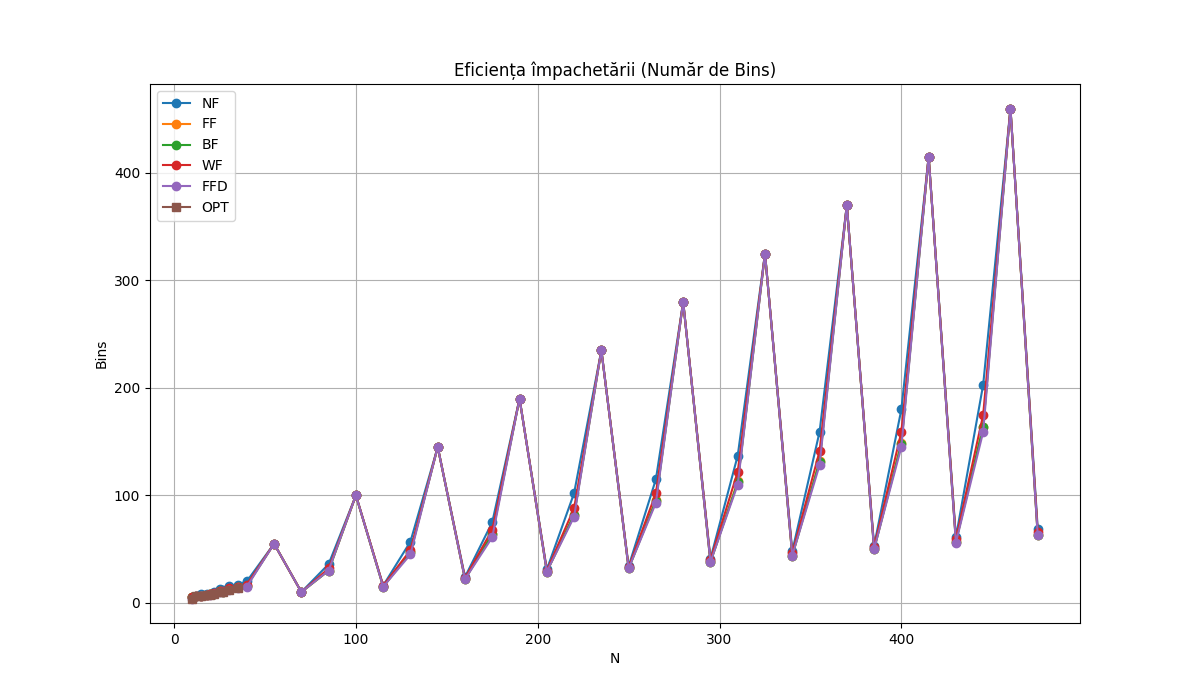
\includegraphics[width=0.9\textwidth]{grafic_bins.png}
\caption{Comparația numărului de containere utilizate în funcție de dimensiunea intrării ($n$). Se observă variația mare cauzată de cele trei tipuri de distribuții.}
\label{fig:bins}
\end{figure}

\begin{figure}[H]
\centering
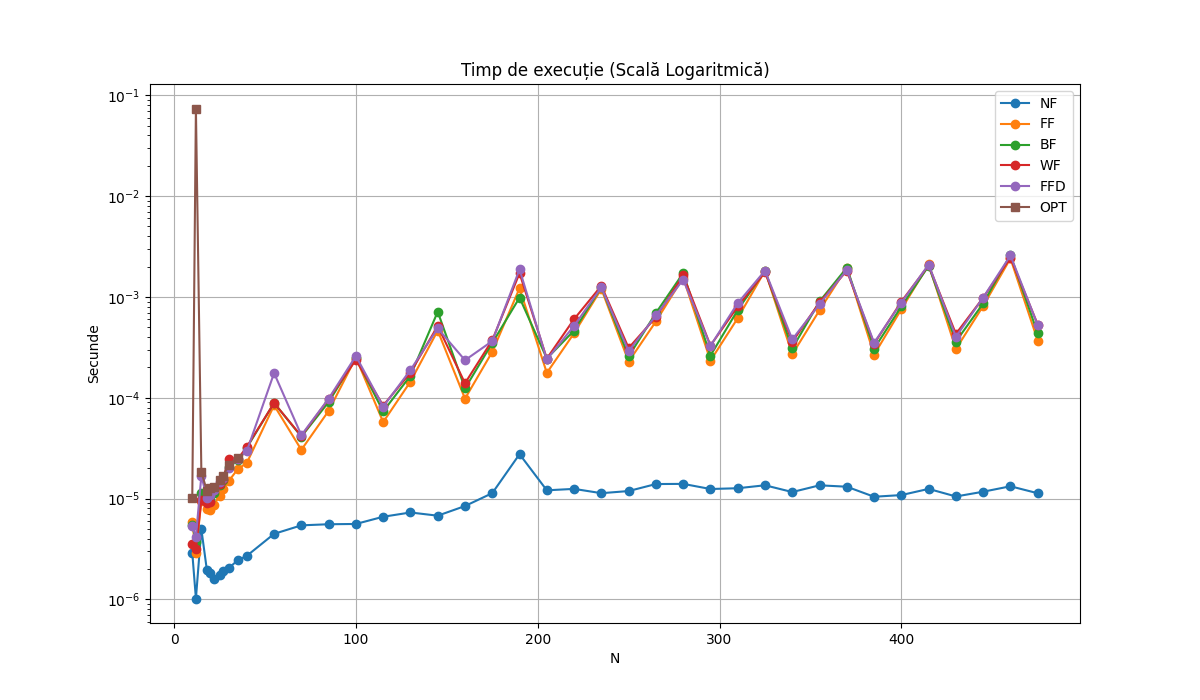
\includegraphics[width=0.9\textwidth]{grafic_timp.png}
\caption{Comparația timpilor de execuție (scară logaritmică). Next Fit rămâne constant rapid ($O(n)$), în timp ce ceilalți algoritmi cresc cu $O(n^2)$.}
\label{fig:time}
\end{figure}

\subsection{Interpretarea Rezultatelor}

\textbf{1. Calitatea soluțiilor:}

FFD a demonstrat cele mai bune rezultate dintre algoritmii de aproximare, atingând optimul în toate testele mici verificabile. Pentru testele cu distribuție uniformă, FFD a economisit consistent 15-25\% din containere comparativ cu NF.

\textbf{2. Comportament pe distribuții specifice:}

\begin{itemize}
    \item \textbf{Obiecte mari ($>50\%$ din capacitate):} Toți algoritmii performează identic, fiecare obiect necesitând propriul container. În acest caz, diferența constă doar în timpul de execuție.
    \item \textbf{Obiecte mici ($<25\%$ din capacitate):} Diferențele între algoritmi sunt reduse, deoarece există multe posibilități de combinare. FFD și BF performează ușor mai bine.
    \item \textbf{Distribuție uniformă:} Aici se observă cele mai mari diferențe între algoritmi. FFD excelează prin plasarea strategică a obiectelor mari primele.
\end{itemize}

\textbf{3. Timpii de execuție:}

\begin{itemize}
    \item NF este cel mai rapid ($O(n)$), menținându-se sub 0.00003s chiar și pentru $n = 475$.
    \item FF, BF, WF, FFD au timpi similari, conformi cu complexitatea $O(n^2)$ în implementarea naivă.
    \item Backtracking devine impracticabil peste $n = 35$, cu timp exponențial.
    \item Variațiile în timpii FF/BF/WF se datorează diferitelor distribuții - mai mulți pași de căutare pentru distribuții favorabile combinărilor.
\end{itemize}

\textbf{4. Valori neașteptate și explicații:}

\begin{itemize}
    \item La $n = 12$, backtracking a durat 0.074s, semnificativ mai mult decât pentru $n = 10$ sau $n = 15$. Aceasta se explică prin configurația specifică a greutăților care a generat un arbore de căutare mai larg, unde FFD nu a atins limita inferioară direct.
    \item Testele cu obiecte mari (unde toți algoritmii dau $n$ containere) au timpi mai mici pentru FF/BF/WF, deoarece căutarea se termină imediat (niciun container existent nu poate primi încă un obiect).
    \item Vârfurile din graficul de timp (ex: $n = 190, 325$) corespund testelor cu obiecte mari, unde numărul mare de containere deschise ($n$ containere) generează mai multe iterații în buclele de căutare.
\end{itemize}

%==============================================================================
\section{Concluzii}
%==============================================================================

În urma studiului comparativ realizat, formulăm următoarele recomandări practice pentru abordarea problemei Bin Packing:

\subsection{Alegerea Algoritmului în Funcție de Context}

\begin{itemize}
    \item \textbf{Pentru aplicații în timp real / streaming:} Recomandăm \textbf{Next Fit} când obiectele sosesc continuu și trebuie procesate imediat, cu resurse minime de memorie. Acceptăm calitatea mai slabă a soluției în schimbul vitezei $O(n)$ și spațiului $O(1)$.
    
    \item \textbf{Pentru cazul general (offline):} Recomandăm \textbf{First Fit Decreasing} ca alegere implicită. Oferă cel mai bun compromis între calitatea soluției (garanție teoretică $\frac{11}{9} \cdot OPT$ și performanță practică aproape optimă) și eficiența computațională.
    
    \item \textbf{Pentru instanțe mici ($n \leq 30-35$):} Dacă soluția optimă este critică și timpul nu este o constrângere strictă, putem folosi \textbf{backtracking optimizat} cu paralelizare.
    
    \item \textbf{Pentru obiecte predominant mari ($>50\%$ din capacitate):} Oricare algoritm produce același rezultat ($n$ containere). Alegem NF pentru viteză maximă.
    
    \item \textbf{Pentru obiecte predominant mici:} FF sau BF sunt suficiente, sortarea din FFD aduce beneficii marginale în acest caz.
\end{itemize}

\subsection{Compromisuri și Trade-off-uri}

Problema Bin Packing ilustrează excelent trade-off-urile fundamentale din algoritmică:
\begin{itemize}
    \item \textbf{Timp vs. Calitate:} Putem obține soluția optimă, dar doar pentru instanțe mici (complexitate exponențială). Pentru instanțe mari, acceptăm soluții aproximative.
    \item \textbf{Online vs. Offline:} Algoritmii offline (FFD) oferă rezultate mai bune, dar necesită cunoașterea întregii intrări în avans.
    \item \textbf{Simplitate vs. Performanță:} NF este extrem de simplu dar oferă garanții slabe; FFD necesită sortare dar oferă garanții excelente.
\end{itemize}

\subsection{Îmbunătățiri Posibile}

Pentru rezultate și mai bune în aplicații practice, se pot considera:
\begin{itemize}
    \item Implementarea FF/BF/WF cu arbori binari de căutare echilibrați pentru $O(n \log n)$.
    \item Algoritmi metaeuristici (Algoritmi Genetici, Simulated Annealing) pentru instanțe mari unde se dorește apropierea de optim.
    \item Branch and Bound cu limite inferioare mai strânse pentru extinderea soluției exacte la instanțe mai mari.
    \item Combinarea euristicilor: rularea mai multor algoritmi și alegerea celui mai bun rezultat.
\end{itemize}

%==============================================================================
\section*{Anexă: Codul Complet Backtracking}
%==============================================================================

\begin{tcolorbox}[colback=blue!5!white, colframe=blue!75!black, title={\faCode\ Implementarea Completă Backtracking cu Paralelizare}, breakable]
\begin{lstlisting}[language=Python, basicstyle=\ttfamily\scriptsize]
from multiprocessing import Pool
import math

def _bt_worker(args):
    # procesare paralela a unui subarbore
    weights, C, start_idx, bins, current_best = args
    n = len(weights)
    best = [current_best]

    def solve(idx, bins):
        if idx == n:
            best[0] = min(best[0], len(bins))
            return

        # Pruning
        if len(bins) >= best[0]:
            return

        # Evitam duplicate - memoram capacitatile incercate
        used = set()
        for i in range(len(bins)):
            if bins[i] >= weights[idx] and bins[i] not in used:
                used.add(bins[i])
                bins[i] -= weights[idx]
                solve(idx + 1, bins)
                bins[i] += weights[idx]

        # Deschidem un container nou
        bins.append(C - weights[idx])
        solve(idx + 1, bins)
        bins.pop()

    solve(start_idx, bins[:])
    return best[0]

def backtracking_optimal(weights, C):
    # Sortam descrescator pentru pruning
    weights = sorted(weights, reverse=True)
    n = len(weights)

    # Calculam lower bound (suma / capacitate)
    total_w = sum(weights)
    lb = math.ceil(total_w / C)

    # Upper bound initial de la FFD
    ub = first_fit_decreasing(weights, C)

    if lb == ub:
        return ub

    # Cate nivele expandam inainte de paralelizare
    PAR_LEVEL = 2
    tasks = []

    def generate_prefixes(idx, bins):
        # prefixe pentru paralelizare
        if idx == PAR_LEVEL:
            tasks.append((weights, C, idx, bins[:], ub))
            return

        used = set()
        for i in range(len(bins)):
            if bins[i] >= weights[idx] and bins[i] not in used:
                used.add(bins[i])
                bins[i] -= weights[idx]
                generate_prefixes(idx + 1, bins)
                bins[i] += weights[idx]

        bins.append(C - weights[idx])
        generate_prefixes(idx + 1, bins)
        bins.pop()

    generate_prefixes(0, [])

    if not tasks:
        return ub

    # Executam task-urile in paralel
    with Pool() as p:
        results = p.map(_bt_worker, tasks)

    return min(results)
\end{lstlisting}
\end{tcolorbox}

%==============================================================================

\begin{thebibliography}{9}

\bibitem{garey1979computers}
Garey, M. R., \& Johnson, D. S. (1979). \textit{Computers and intractability: A guide to the theory of NP-completeness}. W.H. Freeman and Company.

\bibitem{dosa2007tight}
Dósa, G. (2007). The tight bound of First Fit Decreasing bin-packing algorithm is $FFD(I) \leq 11/9 OPT(I) + 6/9$. In \textit{Combinatorics, Algorithms, Probabilistic and Experimental Methodologies} (pp. 1-11). Springer.

\bibitem{coffman1996approximation}
Coffman Jr, E. G., Garey, M. R., \& Johnson, D. S. (1996). Approximation algorithms for bin packing: A survey. In \textit{Approximation algorithms for NP-hard problems} (pp. 46-93). PWS Publishing Co.

\bibitem{johnson1973near}
Johnson, D. S. (1973). Near-optimal bin packing algorithms. Doctoral dissertation, Massachusetts Institute of Technology.

\bibitem{korte2012combinatorial}
Korte, B., \& Vygen, J. (2012). \textit{Combinatorial optimization: Theory and algorithms} (5th ed.). Springer Science \& Business Media.

\bibitem{geeksforgeeks2024binpacking}
GeeksforGeeks. (2024). Bin Packing Problem (Minimize number of used Bins). Accesat la 5 ianuarie 2026, de la \url{https://www.geeksforgeeks.org/bin-packing-problem-minimize-number-of-used-bins/}

\end{thebibliography}

\end{document}
